\documentclass[a4paper,10pt]{article}
%opening
\usepackage{graphicx}

\title{GoMule User Guide.}
\author{Silospen}

\begin{document}

\maketitle
\clearpage
\tableofcontents
\clearpage

\section{Introduction}

GoMule is designed as a muling application. Muling is the movement of items from one character to another, either in Diablo 2 or outside of the game. In this case, GoMule allows character items to be moved between characters without the Diablo 2 application.

\subsection{File Types}

There are 3 basic file types:

\begin{itemize}
 \item D2S: Standard Diablo 2 character file
 \item D2X: ATMA Diablo 2 stash
 \item ORG: ATMA Diablo 2 character file backup
\end{itemize}

\subsubsection{D2S}

The D2S file is the format created by blizzard which holds the Diablo 2 character information. This ranges from current stat and skill allocation, to quest data and item information. GoMule reads from and edits these files, resulting in transferral of items and displaying of character details.

\subsubsection{D2X}

The Diablo 2 character has only a small amount of space to store items. Thus, a more appropriate way of storing items was devised by the creator of ATMA, resulting in the D2X file. This is commonly called a ``stash''. You can think of a D2X as an unlimited extended stash for items, giving you the ability to store a much larger number of items.

\subsubsection{ORG}

ORG files are copies made at regular intervals to ensure that any data which is lost can be restored. There should be a .ORG file for every .D2S file and restoring them simply involves renaming the files from .ORG to .D2S.


\subsection{Project Based Muling}

GoMule uses a system called 'projects' to make it easier for the user to organise their characters and stashes. It also allows a complete separation of different items and characters, such as HC vs SC, twinked vs untwinked etc.

If you do not wish to use projects, you don't have to do anything. The default project, 'GoMule', will be used by default and you don't have to worry about changing projects or anything along those lines. If you're an intrigued user, however, you should at least try out projects, especially if you have a variety of Diablo 2 projects going on!

\subsubsection{Example Setup}

So, lets say you have a number of Diablo 2 projects going on, such as: 

\begin{itemize}
 \item PVP Project
 \item MF'ing various bosses
 \item Untwinked HC singlepass tournament
\end{itemize}

And lets imagine you have stashes such as:

\begin{itemize}
 \item Large unique item stash
\item Large set item stash
\item Large misc item stash
 \item Collection of PVP characters
\item Collection of MF characters
 \item Single stash for finds in the HC tourney
\item Single character from HC tourney
\end{itemize}


\subsubsection{Example Project Layout}

I would setup my projects like this:\newline


\textbf{``MF'' Project, containing:}
\begin{itemize}
 \item Large unique item stash
\item Large set item stash
\item Large misc item stash
\item Collection of MF characters
\end{itemize}

\textbf{``PVP'' Project, containing:}
\begin{itemize}
 \item Large unique item stash
\item Large set item stash
\item Large misc item stash
 \item Collection of PVP characters
\end{itemize}

\textbf{``HCTourney'' Project, containing: }
\begin{itemize}
 \item Single stash for finds in the HC tourney
\item Single character from HC tourney
\end{itemize}

This solution may not be the best for you, but it allows you to isolate your items, characters and stashes, so you only have to consider a small number at a time. With the case of the tournament project in this example, it is totally isolated from all of your other chars/stashes/items, so there is no chance of an accidental item crossing into the tournament stash. 

Anyway, have a look at it. You can always not use it if you want.


\section{Obtaining and Installing GoMule}

\subsection{Obtaining}

If you have found this guide, you should also have found a link to GoMule

\subsection{Installation}

GoMule requires java. If GoMule doesn't work it is likely you need to download java from sun.java.com

Download the latest.zip folder and extract it. Inside there should be a number of folders and a file named ``GoMule.jar''. Double click on this folder. For the command line monkeys, run ``java -jar GoMule.jar''.

\section{Normal GoMule Operation}

This is the screen which you should see when running GoMule:

\begin{figure}[htp]
\centering
 \includegraphics[width=140mm]{baseGUI.png}

\end{figure}

Welcome to the main GUI. It is split into 3 separate areas which have been labeled and will be examined in depth:
\begin{itemize}
 \item GoMule Tool/Menu Bar
 \item GoMule Left Pane
 \item GoMule Right Pane
\end{itemize}

\section{GoMule Tool/Menu Bar}

\begin{figure}[htp]
\centering
 \includegraphics[width=140mm]{baseGUITop.png}
\end{figure}

\subsection{Character (D2S) Operations}

\subsubsection{Open Char}

This allows a character to be opened in GoMule. Once a character has been opened, it is then accessible through the char/stash view. Multiple characters can be selected in the open file window, using standard shift + click, ctrl + click and ctrl + A methods.

\subsubsection{Add Char}

This adds a character to the GoMule char/stash view without opening the character up. Again, multiple files can be selected. This function is useful when you wish to add a large number of characters to GoMule's char/stash view, but don't wish to open them all. 

\subsection{Stash (D2X) Operations}

\subsubsection{New Stash}

Creates a new, empty item stash and adds it to the char/stash view.

\subsubsection{Open Stash}

Same as ``Add Char'', but with stashes. 

\subsubsection{Add Stash}

Same as ``Add Char'', but with stashes.

\subsection{Save All}

Saves all of the currently open stashes/chars.

\subsection{Reload All}

Reloads all the currently open stashes/chars.

\subsection{File Menu}

This actually just contains what's already on the toolbar. It just looks odd if a program doesn't have one ;)

\subsection{Project Menu}

Contains the project preferences box.

\subsubsection{Project Preferences}

\begin{figure}[htp]
\centering
 \includegraphics[width=140mm]{projOpts.png}
\end{figure}

The project options are mainly self explanatory, apart from ``Ignore common items on pickup''. When using multiple pickup buttons, certain items are ignored. These include:

\begin{itemize}
 \item In the inventory: Cube, Tomes, Keys, Charms
 \item In the stash: Cube
 \item All equipped items
 \item All items on the belt
\end{itemize}

\subsection{About Menu}

Some thank-you's and credits.

\section{GoMule Left Pane}

The left pane of GoMule is concerned with project control.

\begin{figure}[htp]
\centering
 \includegraphics[width=140mm]{leftpane.png}
\end{figure}

\section{Project Selector Box}

Using this dropdown box you can select any projects which you have added. The default project is GoMule. Please see the projects section for more information on projects.

\subsection{Char/Stash View}

This is a fast access panel to all of the characters and stashes which you have opened with GoMule. When you open a character or a stash, it is automatically added here. Then to open it again, simply double click on it here.

\subsubsection{All Item View}

The GoMule all item view is intended to allow a user to easily find items. When All is clicked on, all of the chars/stashes in the current project (shown in the Char/Stash view) are read and all of the items are placed into a stash. This stash is then displayed.

The stash cannot be added to, but items can be taken from it. If an item is taken from the all item stash, it is taken from it's location on whichever char/stash it exists in and placed on the clipboard. 

\subsection{Project Controls}

The controls are fairly self explanatory. This is where you add, delete and clear all the chars/stashes from a GoMule project. Note that deleting a project DELETES THE CLIPBOARD TOO!

\subsubsection{Proj Flavie Report}

This creates a flavie report of the entire project in the GoMule directory. The name will look like $\langle$projname$\rangle$Report.html.

\subsubsection{Proj Txt Dump}

This performs a txt dump for every char/stash in the project. The dumps will be saved to a folder in your GoMule directory named $\langle$projname$\rangle$Dumps.
\newpage
\section{GoMule Right Pane}

The right pane of GoMule is concerned with item and character control.

\begin{figure}[htp]
\centering
 \includegraphics[width=140mm]{rightpane.png}
\end{figure}

\subsection{Item Clipboard}

The GoMule item clipboard is a location for items in transit. Items to be moved are picked up onto the clipboard then taken off the clipboard when they are dropped. Acts the same as the cursor in Diablo 2, but it allows multiple items to be added to it. It operates on a Last In First Out (LIFO) principle, so the next item you drop will be the last item you placed on the clipboard.

To drop an item further up the clipboard, click the name of the item to drop and then that item will be dropped on the next drop operation.

\subsubsection{GoMule Bank}

The GoMule bank is an unlimited store for gold. Simply place gold from you chars to here to store gold, through the bank interface on the character screens.

\subsubsection{Item View Panel}

This shows an image of the currently selected item in the clipboard. Hover over the item and a popup of the item properties will appear. This allows you to check an item without removing it from the clipboard.

\subsection{Item Control}

These buttons allow you to quickly manipulate items. Note that if the ``Ignore common items on pickup'' box is checked in the project options, certain items will be ignored when using these buttons (see above).

\subsubsection{Pick All}

This is active for both stashes and characters. When you click it, all the items contained in the stash/character will be picked up and placed on the clipboard.

\subsubsection{Drop All}

This is active for both stashes and characters. When you click it, all the items on the clipboard will be placed in the selected character/stash. In the case of a character, all the items that fit will be placed on the character.

\subsubsection{Pickup From}

This is active for only characters. Select from the dropdown box which area you want to pick items up from. Click 'Pickup From...' and all the items in that area will be put on the clipboard.

\subsubsection{Drop From}

This is active for only characters. Select from the dropdown box which area you want to drop items to. Click 'Drop To...' and items will be transferred to the character from the clipboard to that area. If there are too many items, all the items that will fit will be transferred.

\subsection{Output Control}

This is where you can output your character as a flavie report or txt dump. Buttons do what they say. Flavie dumps are saved as $\langle$charname$\rangle$Report.html. Text dumps are saved as $\langle$charname$\rangle$.txt.
\newpage
\section{Muling with Characters}

This is what a character window looks like in GoMule:

\begin{figure}[htp]
\centering
 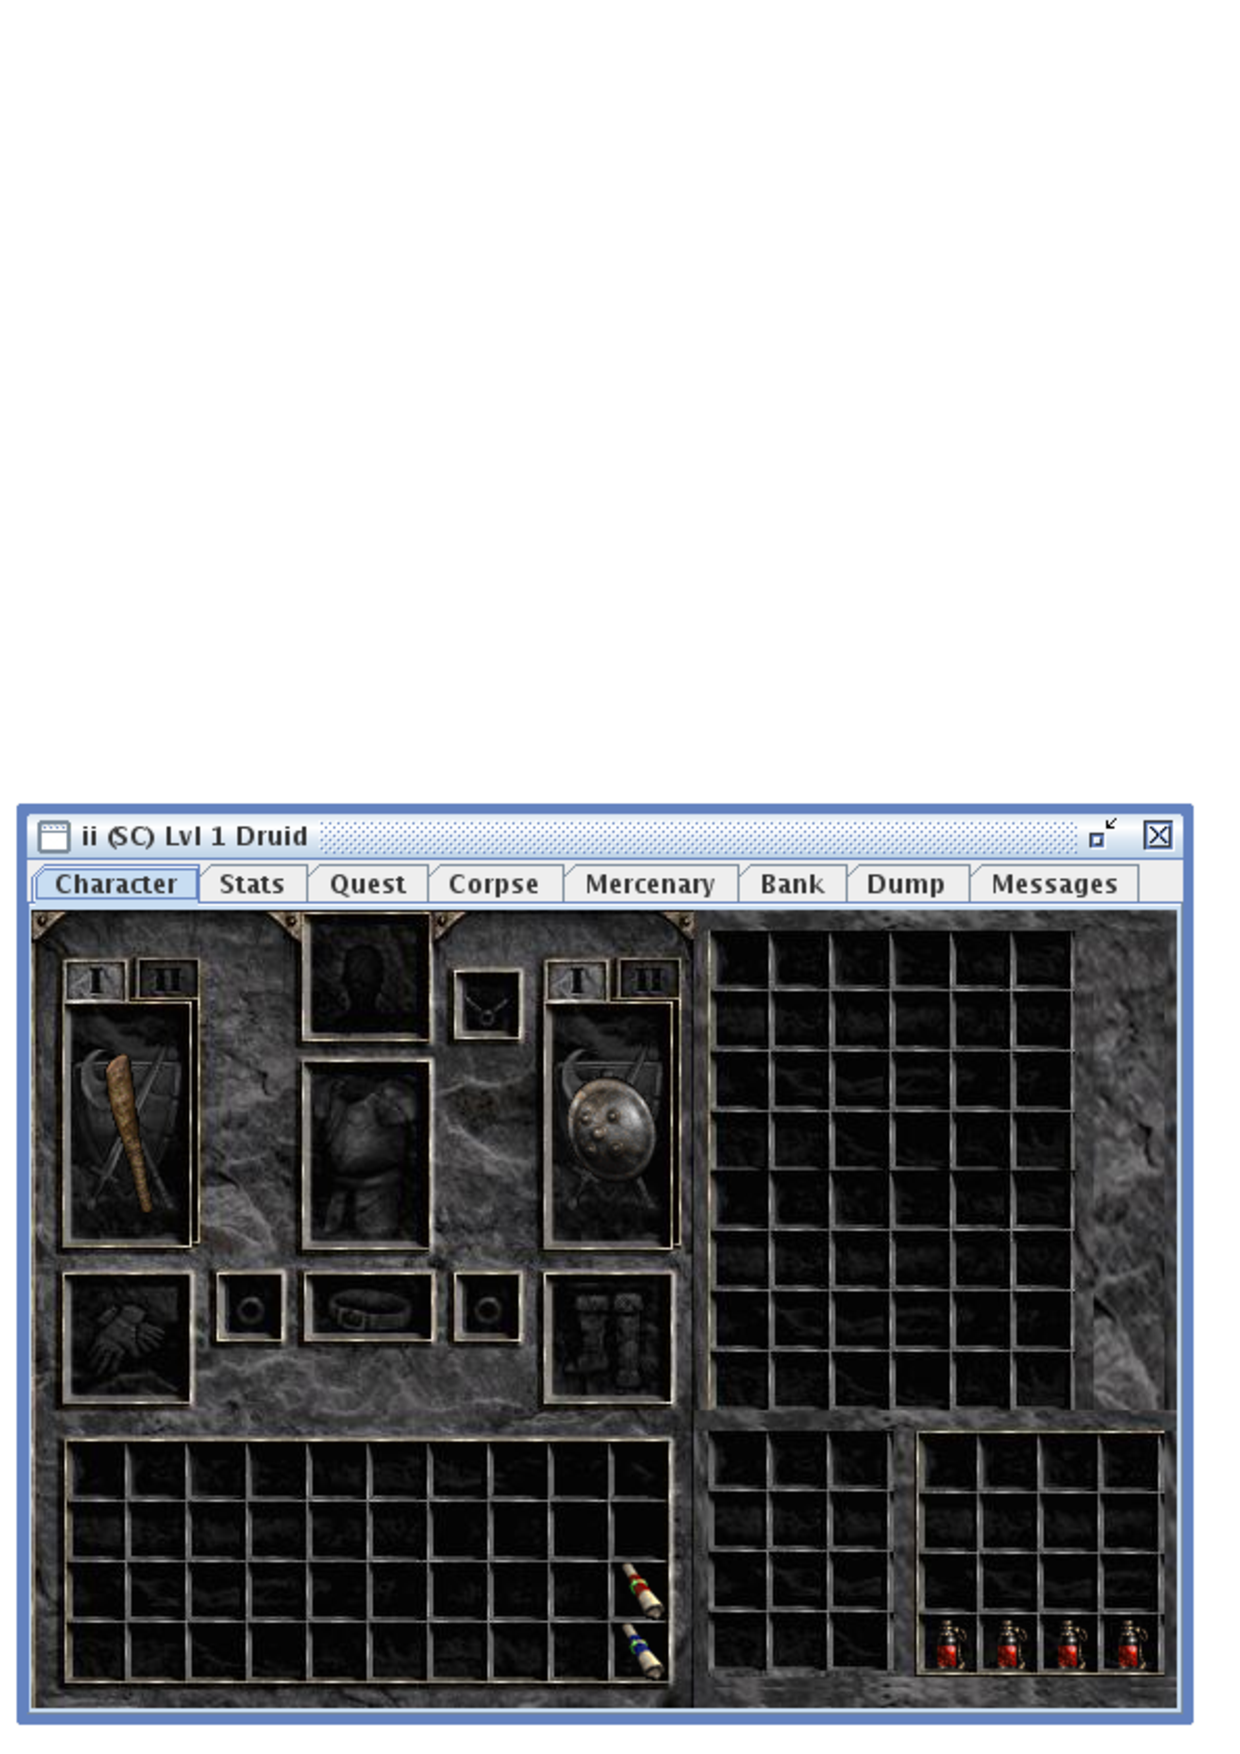
\includegraphics[width=140mm]{char.png}
\end{figure}

The character is accessible through a number of tabs, which will now be explained.

\subsection{Character Tab}

This is your basic item view of your character's inventory, stash, cube and belt. You should recognise it. 

To view the properties of an item, hover over an item and a tooltip with the properties in it will appear.

To move an item, left click on the item. It will now be added to the clipboard. To place it down again, find a suitable location and left click to drop it. Notice how the cursor changes when you are in a valid drop location.

To access weapon switch, click the ``I'' ``II'', just as in game.

\subsubsection{Right Click Menu}

Right clicking on an item will bring up a new menu, containing the options:

\begin{itemize}
 \item Delete?
\item View Item
\end{itemize}

\subsubsection{Delete?}

Removes the item. This is permanent once the character file is saved, so use wisely on items you really do want to delete.

\subsubsection{View Item}

Opens a new window with the item dump in it, in the form of a text dump. This can be selected using the mouse or with ctrl + A, and copied with ctrl + C, allowing a user to show the properties of the item easily, once the dump is pasted somewhere else.

\subsection{Stats Tab}

Shows the current stats of your character as derived by GoMule. Also shows skill point allocations.

\subsection{Quest Tab}

The current quest and waypoint progression of your character.

\subsection{Corpse Tab}

Any items which are on your corpse or on the Diablo 2 cursor are shown here. They are not movable, you'll have to do that in game.

\subsection{Mercenary Tab}

Shows your mercenary with some basic stats. You can give your mercenary items in the normal manner.

\subsection{Bank Tab}

Simple bank interface. You can transfer gold to your char from the clipboard or from your char to the clipboard. ``Gold'' is the gold on the Diablo 2 character inventory screen, ``Gold Stash'' is the gold on the Diablo 2 stash screen.

\subsection{Dump Tab}

Basic text dump of all character information. Copy and paste it if you wish.

\subsection{Messages Tab}

Some tech stuff. This is what you'll see when things go wrong.

\subsection{AutoSave}

Autosave is on, when you close a character using the ``X'', it will be automatically saved.

\section{Muling with Stashes}

This is what a stash window looks like in GoMule:

\begin{figure}[htp]
\centering
 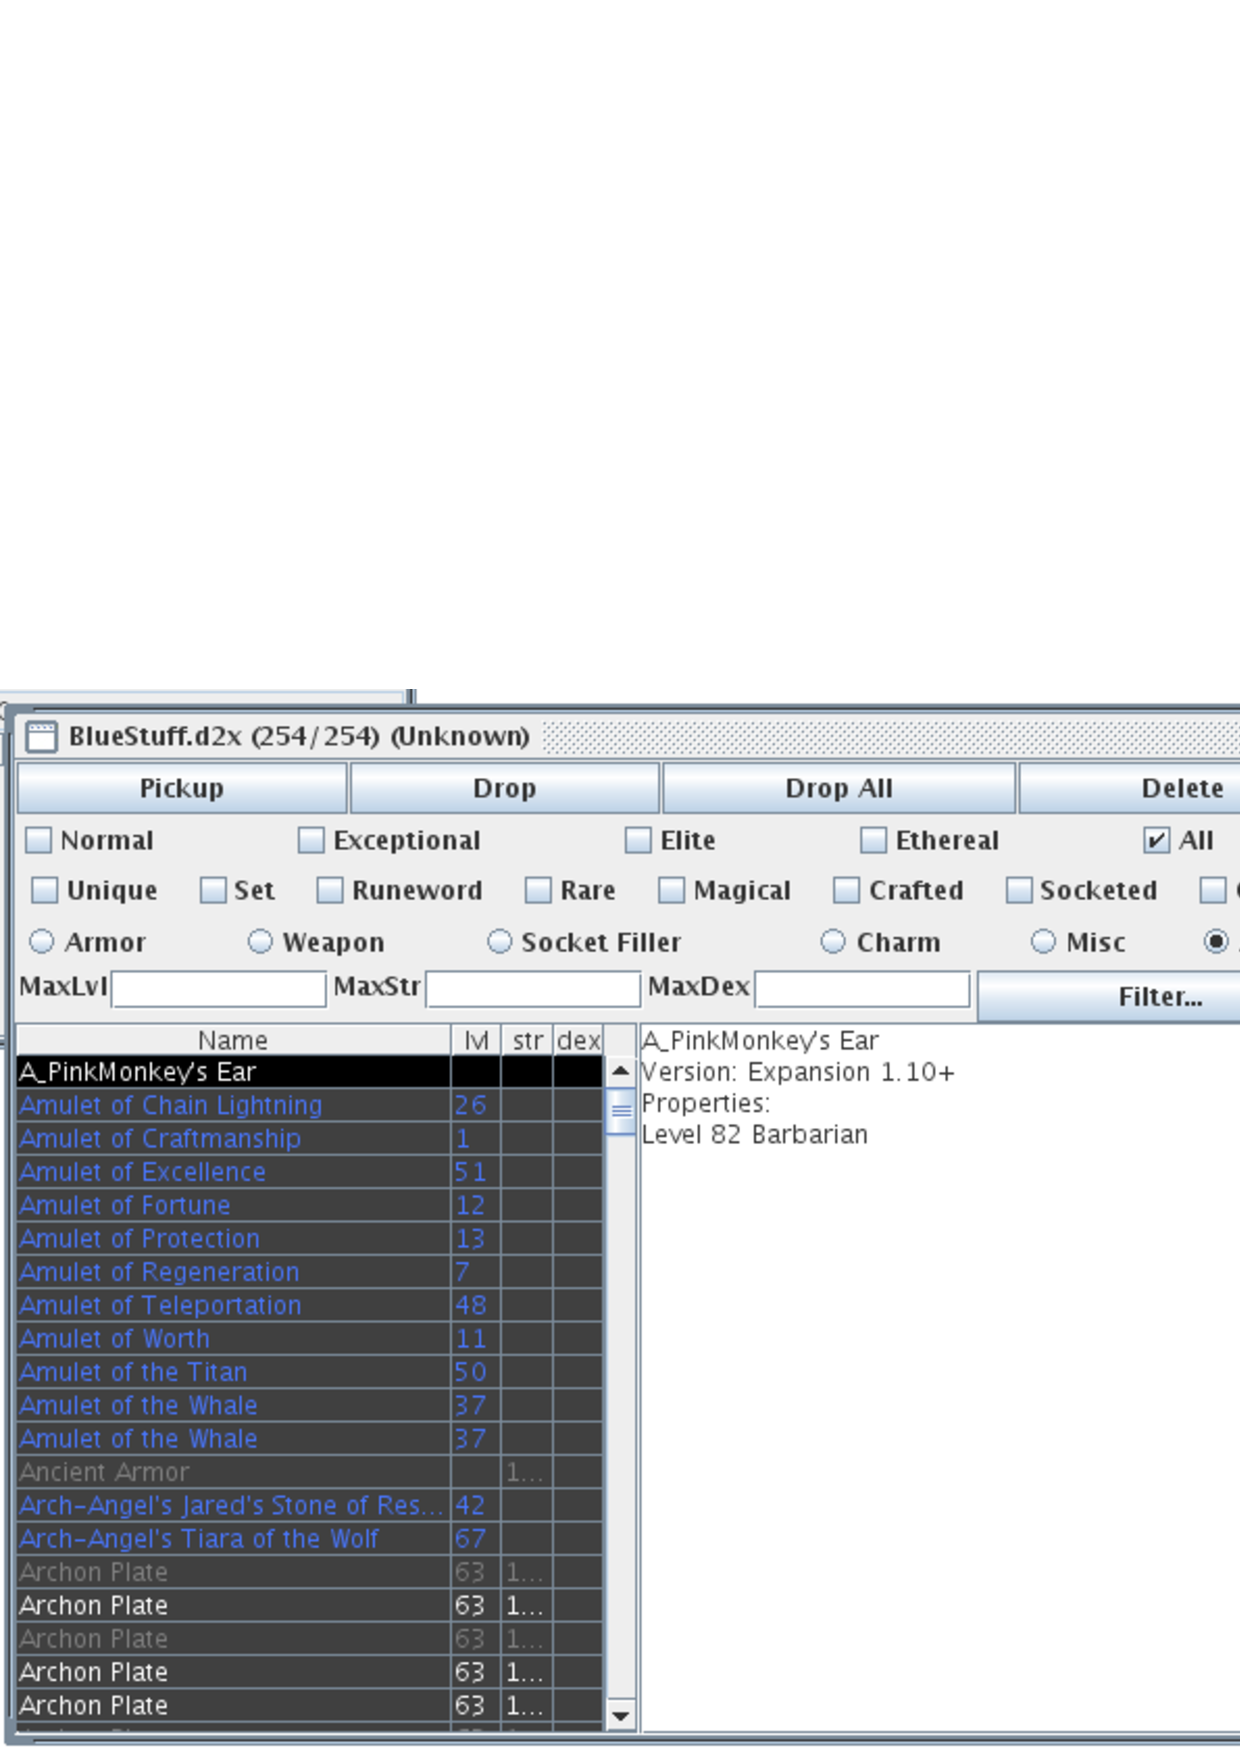
\includegraphics[width=140mm]{stash.png}
\end{figure}

Various buttons and filters will be explained later. There are 2 main panes:

\begin{itemize}
 \item Item Pane
 \item View Pane
\end{itemize}

\subsection{Item Pane}

The item pane is a list of all the items in the stash currently. Clicking on an item will show it's details in the view pane. You can select multiple items using ctrl + click, shift + click or even clicking and dragging your mouse up/down the list. ctrl + A works as well.

You can now pickup an item by double clicking on the name!

Items can be sorted by item name by clicking on the ``Name'' column header, level by clicking on the ``lvl'' column header, etc.

\subsection{View Pane}

Shows the dump of the item information.

\subsection{Filters}

There are various checkboxes and radiobuttons to filter the items in the item pane to allow you to find what you're looking for. This should be self explanatory, play with it a little and you'll get the idea.

The ``MaxLvl'', ``MaxDex'' and ``MaxStr'' fields allow you to filter based on these fields. Just enter a number and the items will be filtered.

\subsection{Buttons}

\subsubsection{Pickup Button}

Takes the item currently selected in the item pane and moves it to the clipboard.

\subsubsection{Drop Button}

Drops the selected item on the clipboard or the last item added to the clipboard into the stash.

\subsubsection{Delete Button}

Deletes the item currently selected in the item pane.

\subsubsection{Delete Dupes Button}

Deletes all items with dual fingerprints.

\subsubsection{Filter... Button}

Opens the custom filter window. The filter looks for items with a user specified property.

There are 3 parts to the custom filter, a String, a Value and Min/Max.

The filter string has to match an item property. For instance, an item with ``20\% Enhanced Damage'' will be returned when the filter string ``Enhanced damage'' is entered. This is also true for partial matches, ``Damage'', ``enhanced'', ``en'', ``dam'' will all return lists containing items with the Enhanced damage property. The string is case insensitive.

The value is the particular value you're looking for. This ties in with the min/max selection. For instance, ``min'' and ``20'' with the previous filter string will return all items in the stash with 20 or greater enhanced damage. ``max'' and ``20'' will return all items in the stash with 20 or less enhanced damage.

The buttons are simple, ``Ok'' performs the filtering, ``Clear'' removes the current filter and ``Cancel'' dismisses the filter window.

Let me be a little more specific about the string search. You may be familiar with a standard text string search in the form of the ``find'' function in firefox/IE/Opera/whatever. Whatever you enter in the find box it will search for, but it can only have an exact match of all of the text entered as the search string. This is the same. ``MF'' will not find items with ``Better Chance of Getting Magic Items'', as it is displayed as ``Better Chance of Getting Magic Items''. ``Better'', ``getting magic'', ``magic items'' all of these and any other combination where the string order is preserved will work. Here's a table:

\begin{table}[h]
\begin{center}
\begin{tabular}{l|p{3.8in}}
What you're looking for & What you should enter (case does \textbf{NOT} matter)\\
\hline
Magic find & Better Chance of Getting Magic Items\\
ED & enhanced damage\\
MF & Better Chance of Getting Magic Items\\
cold res & Cold Resist \\
ias & Increased attack speed\\
\end{tabular}
\end{center}
\end{table}

The table outlines the \textbf{maximum} you should enter as the search query. ``cold res'' is a partial of ``cold resist'' and so it will return all items with ``cold resist'' as a stat. ``increased attack'' will return items with IAS as it is a partial match on ``increased attack speed''. ``Increased speed'' will not provide a match, because although it is a partial string of ``increased attack speed'', the order has been lost!

\subsubsection{Filtering non numerical stats}

There is also the possibility of looking for non numerical stats. If we look at the item Fortitude:


\begin{verbatim}
 Fortitude
Superior Archon Plate
Defense: 1515
Indestructible
Required Level: 63
Required Strength: 103
Fingerprint: 0x291b495e
Item Level: 90
Version: Expansion
Properties: 
All Resistances +30
200% Enhanced Defense
\end{verbatim}

Then we can search for all of the following. Here's another table (assumes ``min'' is selected:

\begin{table}[h]
\begin{center}
\begin{tabular}{l|l|l}
What you're looking for & String & Value (case does \textbf{NOT} matter)\\
\hline
Fortitude & Fortitude & (nothing!) \\
Ilvl & Item Level & (any num less than 91)\\
Fingerprint: 0x291b495e & 0x291b495e & (nothing!)\\
Version: Expansion & Expansion & (nothing!)\\
\end{tabular}
\end{center}
\end{table}

Get it? So if you're looking for something without a specific integer value, just clear the value box. Internally this sets it to -1337, so placing -1337 as the value will have the same effect.

For stats such as poision damage over time, where there is more than one number, GoMule will always filter based on the first number in the property. ``20\% Chance to cast level 15 Chilling Armor when struck'' will be performing the val search on the ``20\%'' and ignoring the ``15''.

Again, this is still the \textbf{maximum} you should enter as the search query. ``em lev'', ``item l'', ``m level'' will all return the ``item level''. ``print'', ``finger'' will still return fingerprint, ``fort'' will get ``fortitude''. It doesn't have to be the whole thing, only a partial string.

I hope that helps you understand :) There should be a box to select stats from. But I'm too lazy to code it, as you've already been informed by GoMule itself.

\section{Known Issues}

As GoMule is an open source project, it is entirely tested and improved by its user base. As such, there are a few issues that are currently affecting GoMule.

\subsection{None so far...}

As this is a new release of the beta, I am not currently aware of any serious issues.

\section{That's it.}

I hope you enjoy GoMule. Feel free to send feedback to silospen@gmail.com

\end{document}
